
%(BEGIN_QUESTION)
% Copyright 2007, Tony R. Kuphaldt, released under the Creative Commons Attribution License (v 1.0)
% This means you may do almost anything with this work of mine, so long as you give me proper credit

If the feedwater control valve for a boiler is placed in manual and then a ``step-change'' increase occurs in steam demand, the effect on steam drum water level will look something like this:

$$\includegraphics[width=15.5cm]{i01799x01.eps}$$

It seems quite normal that water level would ramp down at a constant rate with a greater steam flow (water being boiled away at a greater rate), liquid level control being a characteristically {\it integrating} process.  However, that initial ``swell'' in water level is quite unexpected to anyone unfamiliar with boiler controls.

\vskip 10pt

The swell results from an immediate reduction in boiler pressure following the increase in steam demand, causing more steam bubbles to form in the tubes and drum.  This artificially swells the volume of fluid in the steam drum before it begins to decrease from the mismatch between higher steam demand and unchanged feedwater flow.

Boiler swell is a problem for drum level control, because it makes the controller ``think'' the water level is moving {\it the wrong direction}.  Explain how this physical effect negatively impacts feedback control, and determine whether the impact is more pronounced in a {\it single-element} or a {\it two-element} feedwater control system.

\underbar{file i01799}
%(END_QUESTION)





%(BEGIN_ANSWER)

By initially moving the ``wrong direction'' in response to a change in steam flow, the drum level feedback signal acts as an {\it inverted} feedforward signal for steam flow, exacerbating the load change's effect instead of preempting it.

\vskip 10pt

Follow-up question: integrating processes such as liquid level typically respond well to aggressive proportional control action (proportional bands of 10\% or less!), but not in this case.  How would you recommend tuning the level controller in a single-element boiler feedwater control system, given the effect of ``swell?''

\vskip 10pt

Challenge question: explain how both two-element and three-element feedwater control helps to mitigate the effect of boiler swell.

%(END_ANSWER)





%(BEGIN_NOTES)

Follow-up answer: instead of relying on high controller gain, the gain must be tempered and more integral action incorporated into the PID tuning.

\vskip 10pt

Two-element feedwater control systems are less impacted by swell than single-element.

\vskip 10pt

Challenge answer: by adding a feedforward to the feedwater control system, any increase in steam flow is fed forward to the feedwater valve.  The inherent ``shrink'' from adding (cool) feedwater to the drum helps balance the ``swell'' caused by increased steam flow, resulting in a more stable (and accurate) drum level signal for the level controller to act upon.

%INDEX% Control, PID tuning: step change (load) revealing negative lead
%INDEX% Physics, heat and temperature: boiler ``swell''

%(END_NOTES)


